\chapter{Лабораторная работа}

\section*{Цель работы}

Целью лабораторной работы является освоение возможностей программы
Microsoft Project по управлению финансовыми потоками на основе анализа
затрат.

\section*{Содержание проекта}

Команда разработчиков из 16 человек занимается созданием карты города на основе собственного модуля отображения. Проект должен быть завершен в течение 6 месяцев. Бюджет проекта: 50 000 рублей.

\section*{Задание 1: работа с таблицей освоенного объема}

Дата отчета: 6 мая

Отобразим таблицу в режиме освоенного объема:

\begin{figure}[H]
	\begin{center}
		
\includegraphics[width=\textwidth]{imgs/task_1_0.png}
	\end{center}
\end{figure}

\textbf{Запланированный объем (ЗО)} -- это те средства, которые были бы затрачены на выполнение задачи в период с начала проекта до выбранной даты отчета, если бы задача точно соответствовала графику и смете.

\textbf{Освоенный объем (ОО)} -- это те средства, которые были бы затрачены на выполнение задачи с самого начала проекта до выбранной даты отчета, если бы фактически выполненная работа оплачивалась согласно смете, т.е. это фактическое количество рабочих часов, оплачиваемых по сметным ставкам.

\textbf{Фактические затраты (ФЗ)} -- это средства, фактически потраченные на выполнение задачи в период с начала проекта до выбранной даты отчета, т.е. это фактическая стоимость задачи или фактическая ставка, умноженная на фактические часы.

\textbf{Отклонение от календарного плана (ОКП)} -- сравнивает сметную стоимость плановой и выполненной работы и позволяет вычислить несоответствие сметы, вызванное исключительно различиями между плановым и фактическим объемом работы. (\textbf{Отрицательный -- проект запаздывает})

\textbf{Отклонение по стоимости (ОПС)} -- сравнивает сметную и фактическую стоимость выполненной работы и позволяет выделить несоответствие сметы, вызванные разницей стоимости ресурсов. (\textbf{Отрицательный -- проект вышел за пределы сметы})

\textbf{Предварительная оценка по завершении (ПОПЗ)} -- в этом поле отображаются ожидаемые общие затраты для задачи, расчет которых основан на предположении, что оставшаяся часть работы будет выполнена в точном соответствии со сметой. ПОПЗ также называется прогнозом по завершении.

\textbf{Затраты по базовому плану (БПЗ)} -- отражает фиксированные затраты и стоимость ресурсов согласно базовому плану (сверхурочные часы считаются по сверхурочной ставке, а обычные по обычной) 

\textbf{Отклонение по завершению (ОПЗ)} -- это разность между БПЗ и ПОПЗ (\textbf{Отрицательный -- имеет место перерасход средств}).

\subsection*{Итоговые характеристики:}

\begin{itemize}
	\item Затраты: 49 942 тысяч рублей
	\item Длительность: 21 неделя
	\item Окончание: 2.08.23
	\item Отклонения от базового плана:
	\begin{itemize}
		\item ОКП положительное -- проект успевает в срок
		\item ОПС положительное -- проект не выходит за пределы сметы
		\item ОПЗ положительное -- отсутствует перерасход средств
	\end{itemize}
\end{itemize}

\section*{Задание 2: работа с отчетами проекта}

Создадим отчет о бюджетной стоимости (Отчет -> Наглядные отчеты -> Отчет о бюджетной стоимости):

\begin{figure}[H]
	\begin{center}
		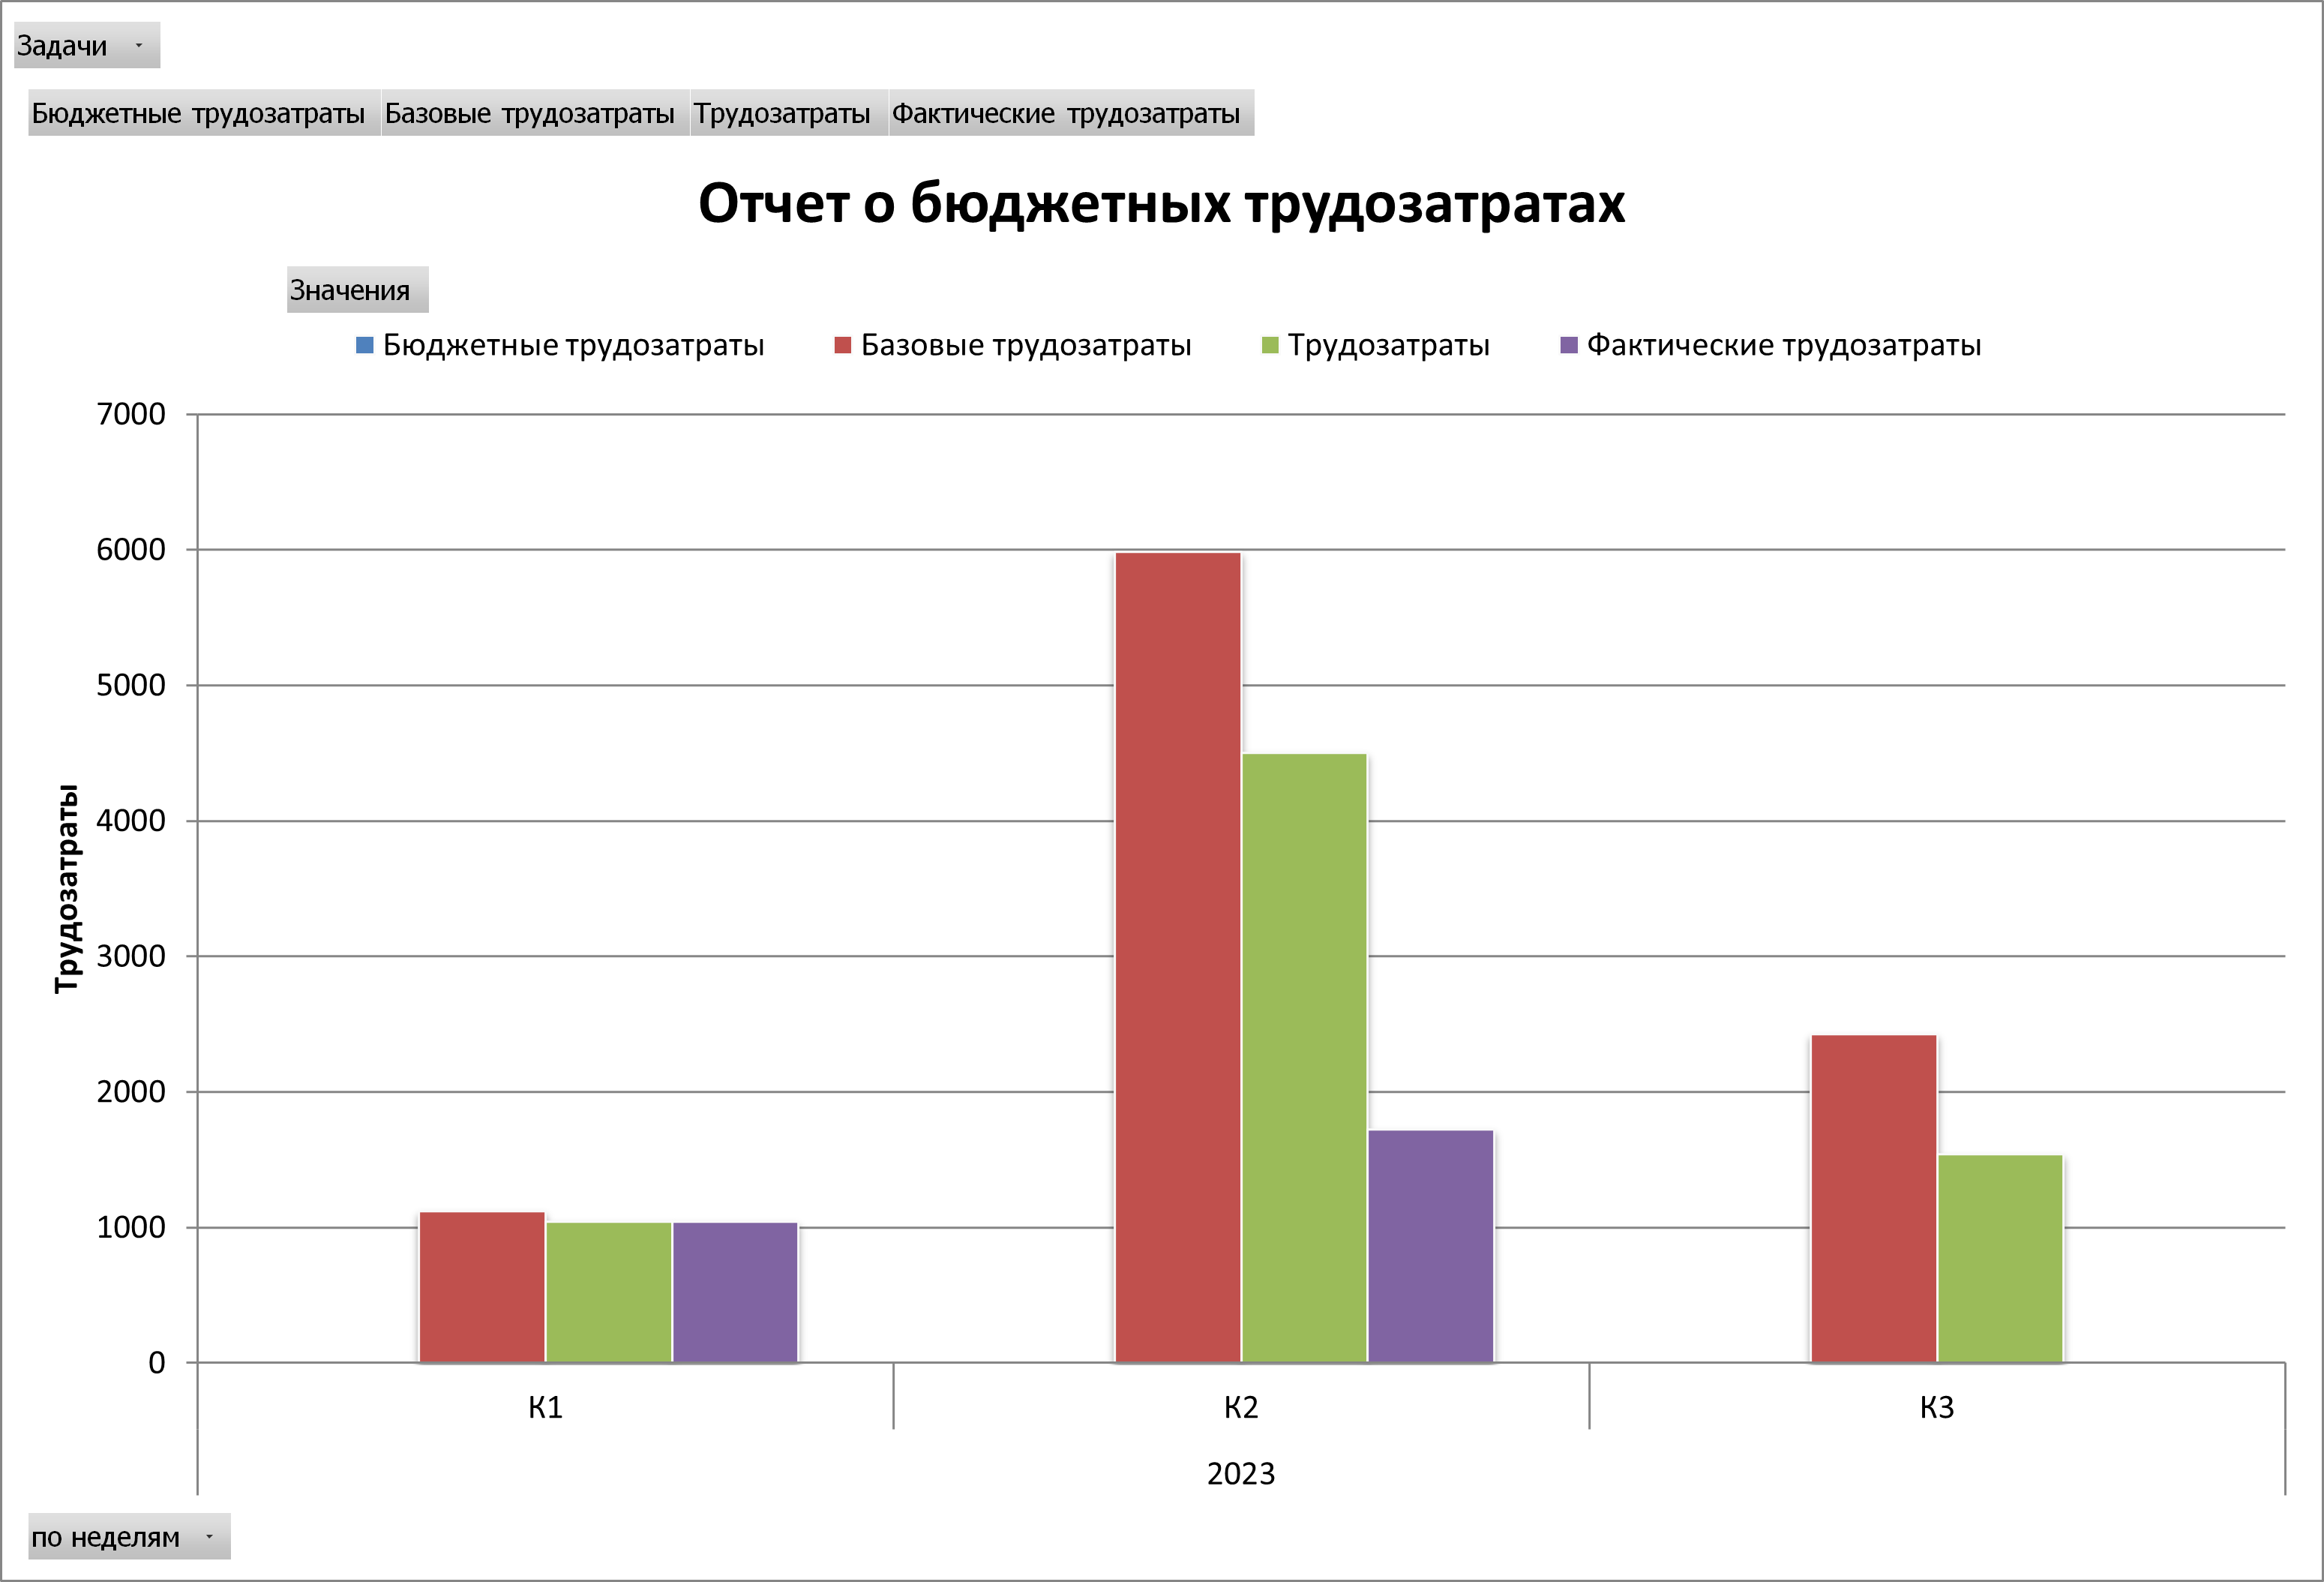
\includegraphics[width=\textwidth]{imgs/task_2_0.png}
	\end{center}
\end{figure}

Отобразим отчет по неделям, а не по кварталам, для этого раскроем кварталы на вкладке <<Использование назначений>>:

\begin{figure}[H]
	\begin{center}
		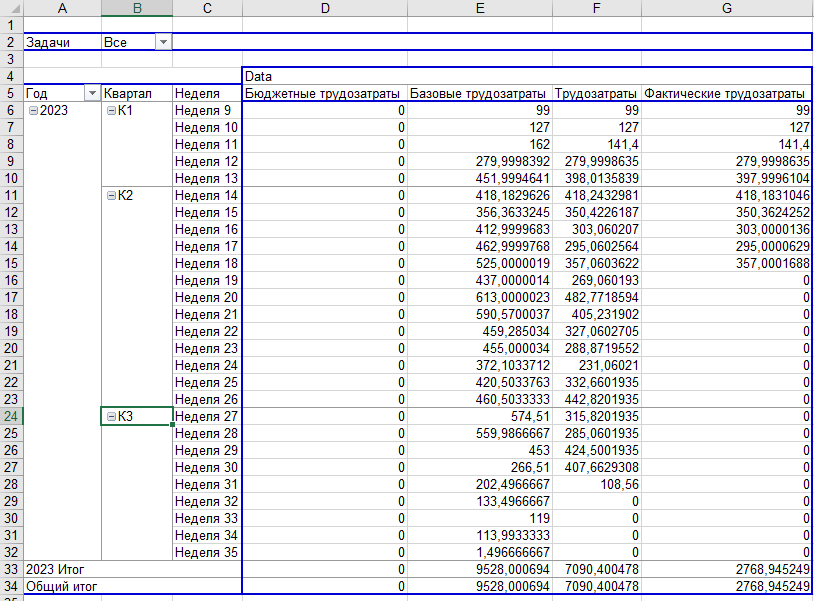
\includegraphics[width=0.7\textwidth]{imgs/task_2_1.png}
	\end{center}
\end{figure}

Получим:

\begin{figure}[H]
	\begin{center}
		
\includegraphics[width=\textwidth]{imgs/task_2_2.png}
	\end{center}
\end{figure}

Исходя из приведенного ниже графика можно сказать, что наибольшие затраты пришлись на 19 неделю. В это время выполнялись задачи <<Наполнение базы объектов>>, <<Создание рабочей версии ядра>> и <<Создание мультимедиа-наполнения>>

Выведем на экран задачи, превышающие бюджетную стоимость.

\begin{figure}[H]
	\begin{center}
		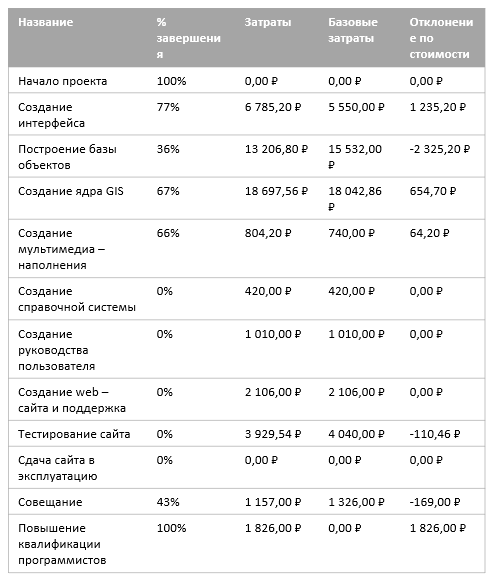
\includegraphics[width=0.65\textwidth]{imgs/task_2_3.png}
	\end{center}
\end{figure}

Из таблицы видно следующее:

\begin{itemize}
	\item отклонение по стоимости создания интерфейса объясняются повышением зарплат программистов, которые занимаются программированием интерфейса (к тому моменту они уже прошли повышение квалификации и им повысили зарплату), и болезнью 3D-аниматора, во время которой художнику-дизайнеру пришлось частично выполнять задачи свои и 3D-аниматора;
	\item отклонение по стоимости создания ядра GIS объясняются повышением зарплат программистов после прохождения повышения квалификации;
	\item отклонение по стоимости построения базы объектов объясняется отказом от аренды сервера и покупкой собственного;
	\item отклонение по стоимости тестирования сайта связаны с поключением к этой задаче программиста-стажера;
	\item отклонение по стоимости создания мультимедиа-наполнения совещаний связаны с повышением зарплаты мультимедиа-корреспондента.
\end{itemize}

\section*{Задание 3: анализ вариантов декомпозиции работ в проекте}

Была проведена декомпозиция задач: если раньше разработка документации и веб-сайта начинались только после создания основного ПО (ядро, БД, интерфейс), то теперь они выполняются параллельно разработке основного ПО. Это позволило сократить срок разработки на 10 дней и расходы на 672 рубля.

До декомпозиции:

\begin{figure}[H]
	\begin{center}
		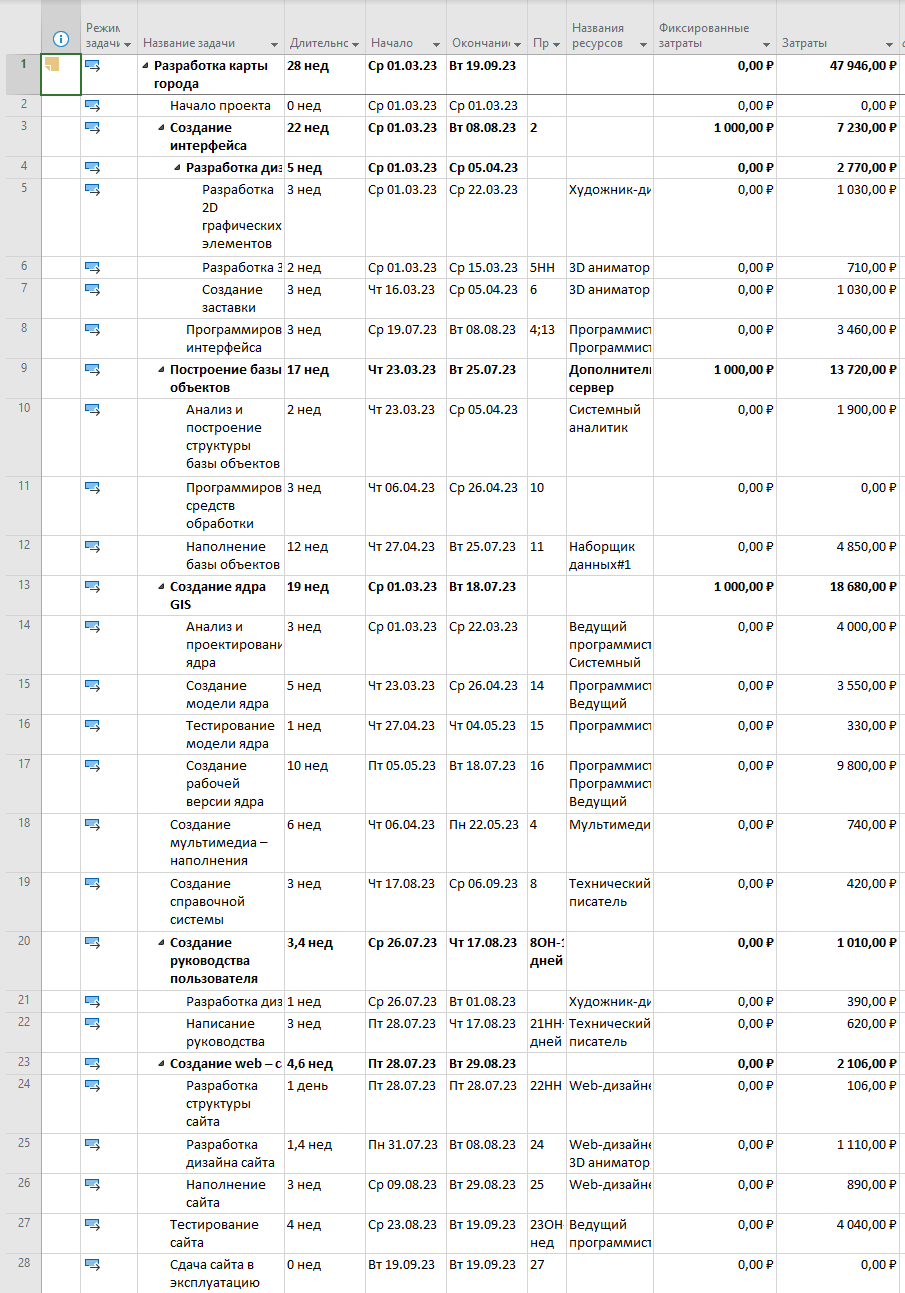
\includegraphics[width=0.85\textwidth]{imgs/task_3_1.png}
	\end{center}
\end{figure}

\begin{figure}[H]
	\begin{center}
		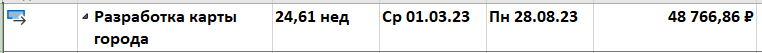
\includegraphics[width=\textwidth]{imgs/task_3_3.png}
	\end{center}
\end{figure}

После декомпозиции:

\begin{figure}[H]
	\begin{center}
		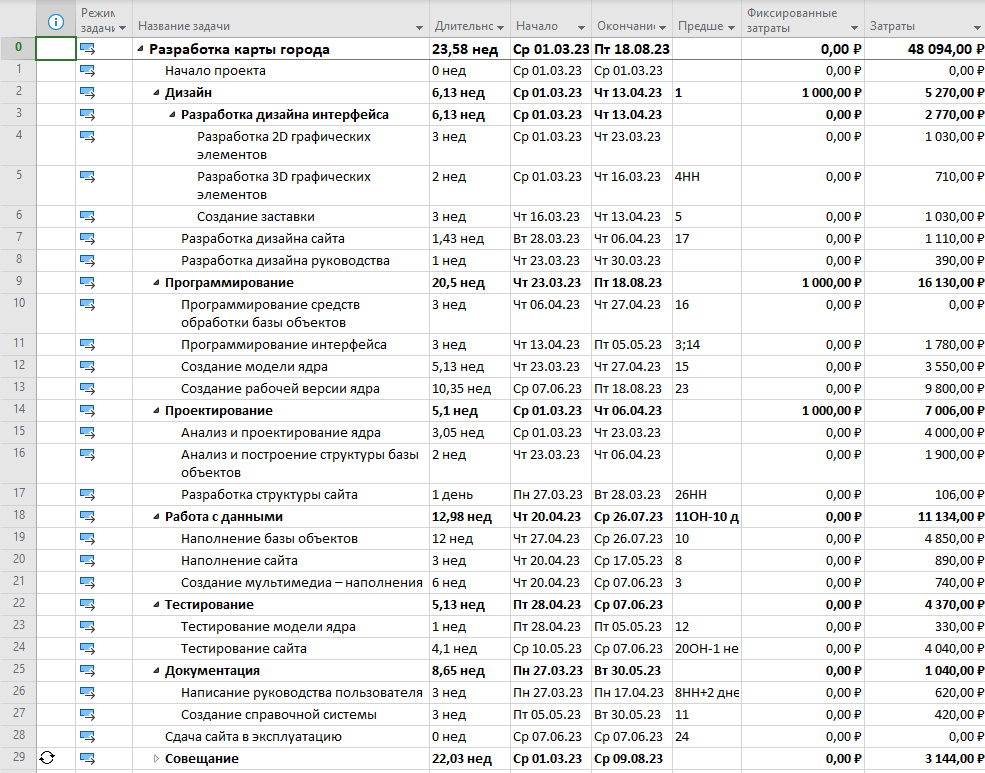
\includegraphics[width=\textwidth]{imgs/task_3_2.png}
	\end{center}
\end{figure}

Этот вариант декомпозиции неидеален: из диаграммы Ганта можно увидеть простои некоторых задач, т. е. они не выполняются непрерывно.